\documentclass[11pt,]{article}
\usepackage{lmodern}
\usepackage{amssymb,amsmath}
\usepackage{ifxetex,ifluatex}
\usepackage{fixltx2e} % provides \textsubscript
\ifnum 0\ifxetex 1\fi\ifluatex 1\fi=0 % if pdftex
  \usepackage[T1]{fontenc}
  \usepackage[utf8]{inputenc}
\else % if luatex or xelatex
  \ifxetex
    \usepackage{mathspec}
  \else
    \usepackage{fontspec}
  \fi
  \defaultfontfeatures{Ligatures=TeX,Scale=MatchLowercase}
\fi
% use upquote if available, for straight quotes in verbatim environments
\IfFileExists{upquote.sty}{\usepackage{upquote}}{}
% use microtype if available
\IfFileExists{microtype.sty}{%
\usepackage{microtype}
\UseMicrotypeSet[protrusion]{basicmath} % disable protrusion for tt fonts
}{}
\usepackage[margin=1.0in]{geometry}
\usepackage{hyperref}
\hypersetup{unicode=true,
            pdftitle={The fecal microbiome as a biomarker for monitoring and predicting remission in Ustekinumab-treated, anti-TNF-alpha refractory Crohn's Disease patients.},
            pdfborder={0 0 0},
            breaklinks=true}
\urlstyle{same}  % don't use monospace font for urls
\usepackage{graphicx,grffile}
\makeatletter
\def\maxwidth{\ifdim\Gin@nat@width>\linewidth\linewidth\else\Gin@nat@width\fi}
\def\maxheight{\ifdim\Gin@nat@height>\textheight\textheight\else\Gin@nat@height\fi}
\makeatother
% Scale images if necessary, so that they will not overflow the page
% margins by default, and it is still possible to overwrite the defaults
% using explicit options in \includegraphics[width, height, ...]{}
\setkeys{Gin}{width=\maxwidth,height=\maxheight,keepaspectratio}
\IfFileExists{parskip.sty}{%
\usepackage{parskip}
}{% else
\setlength{\parindent}{0pt}
\setlength{\parskip}{6pt plus 2pt minus 1pt}
}
\setlength{\emergencystretch}{3em}  % prevent overfull lines
\providecommand{\tightlist}{%
  \setlength{\itemsep}{0pt}\setlength{\parskip}{0pt}}
\setcounter{secnumdepth}{0}
% Redefines (sub)paragraphs to behave more like sections
\ifx\paragraph\undefined\else
\let\oldparagraph\paragraph
\renewcommand{\paragraph}[1]{\oldparagraph{#1}\mbox{}}
\fi
\ifx\subparagraph\undefined\else
\let\oldsubparagraph\subparagraph
\renewcommand{\subparagraph}[1]{\oldsubparagraph{#1}\mbox{}}
\fi

%%% Use protect on footnotes to avoid problems with footnotes in titles
\let\rmarkdownfootnote\footnote%
\def\footnote{\protect\rmarkdownfootnote}

%%% Change title format to be more compact
\usepackage{titling}

% Create subtitle command for use in maketitle
\newcommand{\subtitle}[1]{
  \posttitle{
    \begin{center}\large#1\end{center}
    }
}

\setlength{\droptitle}{-2em}
  \title{The fecal microbiome as a biomarker for monitoring and predicting
remission in Ustekinumab-treated, anti-TNF-alpha refractory Crohn's
Disease patients.}
  \pretitle{\vspace{\droptitle}\centering\huge}
  \posttitle{\par}
  \author{}
  \preauthor{}\postauthor{}
  \date{}
  \predate{}\postdate{}

\usepackage{setspace}
\doublespacing
\usepackage{lineno}
\linenumbers
\renewcommand{\familydefault}{\sfdefault}
\usepackage{graphicx}

\begin{document}
\maketitle

\vspace{35mm}

Running title: Microbiome of Ustekinumab-treated Crohn's Disease
patients.

\vspace{35mm} Matthew K. Doherty\({^2}\), Tao Ding\({^2}\)\({^\alpha}\),
Charlie Koumpouras\({^2}\), Shannon Telesco\({^1}\), Calixte
Monast\({^1}\), and Patrick D. Schloss\({^2}\)\({^\dagger}\)

\(\dagger\) To whom correspondence should be addressed:
\href{mailto:pschloss@umich.edu}{\nolinkurl{pschloss@umich.edu}}

1. Janssen Pharmaceutical Companies of Johnson \({\&}\) Johnson, Spring
House, PA, USA

2. Department of Microbiology and Immunology, University of Michigan,
Ann Arbor, MI, USA

\({\alpha}\) Currently at Department of Biology, New York University,
New York, NY, USA.

\newpage

\subsection{Abstract}\label{abstract}

\emph{Abstract:} Crohn's disease (CD) is a global health concern
characterized by patches of ulceration and inflammation along the
gastrointestinal tract, as well as reduced gut microbial diversity. We
investigated the association between the fecal microbiome and clinical
phenotypes in subjects with moderate to severe CD, refractory to
anti-TNF\({\alpha}\), that was treated with Ustekinumab (UST) in a
double-blinded, placebo-controlled, Phase 2b clinical trial. We
hypothesized that the fecal microbiome would be different between
treatment response groups. Stool samples from 306 subjects, at
screening, were obtained over the course of 22 weeks. The V4 region of
the 16S rRNA gene was amplified and sequenced to determine the structure
of the fecal bacterial communities.

The \({\alpha}\)-diversity of UST treated clinical responders increased
over time, in contrast to nonresponsive subjects. Using Random Forest
models, differences in the fecal microbiome following treatment could
classify patients in remission from those with active disease. The
baseline microbiome and clinical metadata could effectively predict
therapeutic response at week 6, especially for remission. Baseline
\({\alpha}\)-diversity was higher in treated subjects in remission at
week 6. Baseline \({\beta}\)-diversity was different based on response
to UST treatment. Two OTUs, \emph{Faecalibacterium} and
\emph{Bacteroides}, were significantly more abundant in treated subjects
who were in remission at week 6. The fecal microbiome at baseline was
also associated with markers for disease severity, such as Crohn's
Disease Activity Index (CDAI), stool frequency, CRP, fecal lactoferrin,
fecal calprotectin, corticosteroid use, disease duration, and tissue
involvement. The observed baseline differences in fecal microbiota and
changes due to therapeutic response support using the microbiome as a
biomarker for establishing and maintaining CD remission.

\emph{Importance:} Finding biomarkers that give clinicians the ability
to predict response to CD treatment at diagnosis will increase the
likelihood of faster induction and maintenance of remission. The fecal
microbiome could be a useful non-invasive biomarker for directing or
monitoring the treatment of CD patients. OTUs associated with remission
following treatment induction, especially \emph{Faecalibacterium}, could
be biomarkers for successful UST treatment of TNF-\({\alpha}\)
refractory CD patients.

\textbf{Keywords: Crohn's Disease, IBD, fecal microbiome, microbiota,
biologics, prediction, biomarkers, remission, Faecalibacterium,
Ustekinumab, Stelara, machine learning, random forest}

\newpage

\subsubsection{Introduction}\label{introduction}

Crohn's disease (CD), an incurable inflammatory bowel disease (IBD), is
a global health concern causing large economic and healthcare
utilization impacts on society (1--3). CD is characterized by patches of
ulceration and inflammation along the entire gastrointestinal tract,
though mostly the ileum and colon. Currently, individuals with CD are
treated based on disease location and risk of complications using
escalating immunosuppressive treatment, and/or surgery, with the goal of
achieving and sustaining remission (4, 5). Faster induction of remission
following diagnosis reduces the risk of irreversible intestinal damage
and disability (5--7). Ideally, clinicians would be able to determine
personalized treatment options for CD patients at diagnosis that would
result in faster achievement of remission (8). Therefore, recent
research has been focused on identifying noninvasive, prognostic
biomarkers to monitor CD severity and predict therapeutic response
(9--11).

The precise etiology of CD remains unknown, but host genetics,
environmental exposure, and the gut microbiome appear to be involved (1,
12). Individuals with CD have reduced microbial diversity in their guts,
compared to healthy individuals, with a lower relative abundance of
\emph{Firmicutes} and an increased relative abundance of
\emph{Enterobacteraciae} and \emph{Bacteroides}, at the phylum level
(13--17). Additionally, genome-wide association studies of individuals
with CD identified several susceptibility loci, including loci involved
in the IL-23 signaling pathway, which could impact the gut microbiome
structure and function (4, 13, 18--24). If the fecal microbiome can be
used to monitor disease severity and predict response to specific
treatment modalities, then clinicians could use it as a noninvasive tool
for prescribing therapies that result in faster remission (25).

The microbiome has been correlated with a variety of diseases and has
shown promise as a predictive tool for disease outcome for gingivitis
(26), cardiovascular disease (27), \emph{Clostridium difficile}
infection (28--30), and colorectal cancer (31, 32). In relation to IBD,
previous studies have shown that the gut microbiome correlates with
disease severity in new-onset, pediatric CD patients (17, 33).
Additionally, recent studies have shown promise for the microbiome as it
relates to IBD and therapeutic response (34, 35). It remains to be
determined, however, whether the fecal microbiome can predict and
monitor response to therapy in CD (13).

The FDA recently approved Ustekinumab (UST), a monoclonal antibody
directed against the shared p40 subunit of IL-12 and IL-23, for the
treatment of CD (5, 36--38). Given the potential impact of IL-23 on the
microbiome (18--24), we hypothesized that UST treatment may alter the
fecal microbiome and that response to UST could be predicted or
influenced by differences in patients' gut microbiota. We analyzed the
fecal microbiomes of individuals who participated in a double-blinded,
placebo-controlled Phase II clinical trial of UST in treating CD (36).
Using 16S rRNA gene sequence data from these patients' stool samples, we
tested whether the microbiome changed in subjects treated with UST and
if clinical responders had a microbiome that was distinct from
non-responders. We also determined associations between clinical
metadata, disease severity, and the fecal microbiome. Our study
demonstrates that the fecal microbiome is associated with baseline
clinical metadata and that these associations are useful in predicting
and monitoring UST treatment outcome.

\subsection{Results}\label{results}

\textbf{Characteristics of the study population and sequencing results}

We characterized the fecal microbiota in a subset of TNF-\({\alpha}\)
refractory CD patients, with moderate to severe CD, who took part in the
double-blinded, CERTIFI clinical trial (36). Demographic and baseline
disease characteristics of this subset are summarized in Table 1.
Patients were randomly assigned to a treatment group in the induction
phase of the study and at week 8 patients were re-randomized into
maintenance therapy groups based on their induction response (Figure
1A). Subjects provided stool samples at screening (week 0), week 4, week
6, and week 22 post induction for analysis using 16S rRNA gene
sequencing (Figure 1B).

Following sequence curation using the mothur software package (39), we
obtained a median of 13,732 sequences per sample (IQR = 7,863-21,978).
Parallel sequencing of a mock community had an error rate of 0.017\%. To
limit effects of uneven sampling, we rarefied the dataset to 3,000
sequences per sample. Samples from subjects that completed the clinical
trial and had complete clinical metadata were included in our analysis.
Of these samples, 306 were provided prior to treatment as well as 258
provided at week 4, 289 at week 6, and 205 at week 22 post-treatment,
for a total of 1,058 samples.

\textbf{The diversity of the microbiome changes in UST responders}

Given the potential impact of IL-23 pathways on the microbiome (18--22),
we hypothesized that UST treatment would alter the fecal microbiome. The
effects of biologic treatment of IBD on the microbiome are not yet well
described, but are hypothesized to be indirect, as these drugs act on
host factors (4). We tested whether treatment with UST alters the
microbiome by performing a Friedman test comparing
\({\alpha}\)-diversity at each time point within each treatment group
based on subjects' week 22 response status. We included 48 subjects
induced and maintained with UST (20 responders, 28 non-responders) and
14 subjects induced and maintained with placebo (10 responders, 4
non-responders), who provided samples at every time point (Figure 1). As
shown in Figure 2, we saw no significant difference in
\({\alpha}\)-diversity over time in subjects who did not respond at week
22, regardless of treatment. However, the \({\alpha}\)-diversity of week
22 UST responders changed over time (p = 0.005). Multiple comparisons
following the Friedman test showed the inverse Simpson index at week 22
was significantly higher than week 0 (p \textless{} 0.05). No change was
observed in subjects induced and maintained with placebo who responded
at week 22.

\textbf{The microbiome following treatment can distinguish between
treatment outcomes}

Having observed that \({\alpha}\)-diversity increases in subjects who
responded to treatment, we hypothesized that we could use the fecal
microbiome to distinguish between subjects who responded to treatment
from those who did not. A recent study demonstrated a link between the
microbiome and disease activity, where specific microbes were associated
with remission compared to active CD (25). We hypothesized that the
microbiome could be used to monitor response to UST therapy in a similar
manner. We used the AUCRF package in R to develop a random forest
classification model to distinguish between subjects by treatment
response based on their fecal microbiome (32, 40). The study design
resulted in only 75 week 22 stool samples from subjects induced and
maintained with UST, so we focused our analysis on the 220 week 6 stool
samples from subjects induced with UST. As shown in Figure 3, the model
could distinguish week 6 responders from non-responders using week 6
stool samples with an AUC of 0.708 (sensitivity = 0.769, specificity =
0.606). For week 6 remission, using week 6 samples the model had an AUC
of 0.866 (sensitivity = 0.833, specificity = 0.832). We were better able
to distinguish remitters from non-remitters compared to responders from
non-responders. We hypothesize that this is due to the relative nature
of the response criteria compared to the threshold used to determine
remission status, as response was defined as a decrease in a subject's
initial CDAI of 30\% or more, while remission was defined as a CDAI
below the threshold of 150.

\textbf{Prediction of remission based on the microbiome at screening}

Having demonstrated that the microbiome at week 6 following induction
could classify week 6 treatment outcomes, we hypothesized that the week
0 fecal microbiome could predict week 6 response to therapy. To test
this hypothesis, we again used the AUCRF package in R to classify week 6
responders from non-responders, as well as week 6 remitters from
non-remitters, based on the relative abundance of fecal microbiome
community members at week 0, clinical metadata at week 0, and the
combination of microbiome and clinical data (32, 40). We ran these
models on 232 week 0 stool samples from subjects induced with UST. The
optimal models for response and remission at the primary endpoint (Week
6) are shown in Figure 4A and C. Using only microbiome data, the model
predicted response with an AUC of 0.737 (specificity = 0.807,
sensitivity = 0.585). When combining clinical metadata with the
microbiome, the model predicted response with an AUC of 0.745
(specificity = 0.727, sensitivity = 0.744). With respect to week 6
remission, using only fecal microbiome data the model had an AUC of
0.838 (specificity = 0.766, sensitivity = 0.806). Finally, when
combining clinical metadata with the microbiome we achieved an AUC of
0.844 (specificity = 0.831, sensitivity = 0.774) for remission at week
6. Prediction with clinical metadata alone did not perform as well as
models using the week 0 fecal microbiome. Also, the models were again
better able to classify remission compared to response.

The majority of OTUs identified as optimal classifiers in our model for
remission were low in abundance across our cohort (Figure 4B and D).
However, two OTUs appeared to be differentially abundant for subjects in
remission at week 6. The relative abundance of
\emph{Escherichia/Shigella} (OTU00001) appeared lower in remitters
(median = 1.07 IQR = 0.033-3.7) compared to non-remitters (median =
4.13, IQR = 0.667-15.4). Also, the relative abundance of
\emph{Faecalibacterium} (OTU00007) was not only higher in remitters
(median = 7.43, IQR = 1.43-11.9) than non-remitters (median = 0.167, IQR
= 0-5.1), it was present prior to the start of treatment in every
subject who was in remission at week 6 post induction.

\textbf{Comparison of clinical responders and non-responders}

As our random forest models identified OTUs abundant across our cohort
that were important in classifying response and remission, we further
explored differences in the week 0 microbiome that could serve as
potential biomarkers for successful UST treatment. We compared the week
0 microbiomes of all 306 subjects who provided a sample at screening
based on treatment group and response at week 6. With respect to
\({\alpha}\)-diversity, subjects induced with UST and in remission at
week 6 had significantly higher diversity based on inverse Simpson than
non-remitters treated with UST (respective median values = 11.6 (IQR =
4.66-13.9), 6.95 (IQR = 4.4-11.8), p = 0.020). No other treatment or
response groups were significantly different. \({\beta}\)-diversity was
significantly different for response and remission in UST treated
subjects at week 6 (response p = 0.012, week 6 remission p = 0.017).
Wilcoxon rank sum tests were performed on the relative abundance of each
phylum and OTU based on treatment group and week 6 response and then
corrected for multiple comparisons. No phyla were significantly
different by treatment and response (Supplemental Figure 1). No OTUs
were significantly different among subjects receiving placebo for
induction, regardless of response and remission status at week 6. Two
OTUs were significantly more abundant in UST-induced, week 6 remitters
compared to non-remitters; \emph{Bacteroides} (OTU0019) (p = 0.022) and
\emph{Faecalibacterium} (OTU0007) (p = 0.0026), as shown in Figure 5.

\textbf{The baseline microbiome associates with clinical variables}

Since we found associations between week 0 microbial diversity and week
6 response, we hypothesized that there were associations between the
microbiome and clinical variables at baseline that could support the use
of the microbiome as a non-invasive biomarker for disease activity (25).
To test this hypothesis, we compared the week 0 microbiome with clinical
data at week 0 for all 306 samples provided at screening (Supplemental
Table 1). We compared \({\alpha}\)-diversity at baseline to clinical
variables using the inverse Simpson index with Spearman correlation,
Wilcoxon rank sum, or Kruskal-Wallis rank sum, tests where appropriate.
We compared \({\beta}\)-diversity with a PERMANOVA using the adonis
function in the vegan R package. Following multiple comparison
correction, we observed small, but significant correlations for lower
\({\alpha}\)-diversity correlating with higher CDAI (rho = -0.161, p =
0.014), higher frequency of loose stools per week (rho = -0.193, p =
0.003), and longer disease duration (rho = -0.225, p = 0.001).
Corticosteroid use was associated with higher \({\alpha}\)-diversity (p
= 0.001). No significant association was observed between
\({\alpha}\)-diversity and CRP, fecal calprotectin, or fecal
lactoferrin. However, the \({\beta}\)-diversity was significantly
different based on CRP (p = 0.033), fecal calprotectin (p = 0.006), and
fecal lactoferrin (p = 0.004). The \({\beta}\)-diversity was also
significantly different based on weekly loose stool frequency (p=
0.024), age (p = 0.033), the tissue affected (p = 0.004), corticosteroid
use (p =0.01), and disease duration (p = 0.004). No significant
differences in the microbiome were observed for BMI, weight, or sex.

\subsection{Discussion}\label{discussion}

With this study we sought to gain a more detailed understanding of if
and how UST treatment affects the microbiome and to determine whether
the microbiome can be used to identify patients who will respond to UST
therapy. We also aimed to gain a better understanding of the interaction
between the human gut microbiome and CD pathogenesis in adult patients
refractory to anti-TNF-\({\alpha}\) therapies with moderate to severe
CD. We found the fecal microbiome to be useful in uncovering
associations between the microbiome and aspects of CD severity metrics
and treatment outcomes. We also showed that the microbiome of treated
responders changed over time. Finally, we demonstrated that the
microbiome could be useful in predicting remission due to UST therapy,
compared to clinical metadata alone, in our unique patient cohort.

We determined whether or not the microbiome is affected by treatment
with biologics by looking at the microbiome of our CD subjects across
multiple time points during treatment. We observed that the
\({\alpha}\)-diversity of clinical responders increased over time, in
contrast to nonresponsive subjects. This observation could be due to
lower inflammation and changes in disease activity corresponding to
improved health in subjects who responded to UST. We were able to
classify subjects who responded to treatment based on their microbiome
following treatment and were better able to predict remission status
compared to response status. Response may be more difficult to classify
due to the relative nature of a decrease (\textgreater{}30\%) in CDAI
compared to a threshold (CDAI\textless{}150) for remission. We also
addressed whether response to therapy can be predicted with the
microbiome by developing a random-forest model that used relative
microbial abundance data and/or clinical metadata for input. Again, we
were better able to predict remission/non-remission than
response/non-response, using samples provided prior to treatment
induction. These findings are consistent with other studies suggesting
the microbiome could be useful as a biomarker in detecting remission
versus active disease (25).

The presented prognostic model is useful for biomarker discovery and
hypothesis generation about the biology of CD as it relates to the
microbiome. Similar models could be further developed into a clinically
useful prognostic tool. \emph{Faecalibacterium} was the most frequently
occurring OTU in our models. It is associated with health, comprising up
to 5\% of the relative abundance in healthy individuals, and has been
shown to be low in CD patients (13, 15, 41, 42). Each subject induced
with UST and in remission at week 6 had measurable
\emph{Faecalibacterium} present at baseline. This supports the
hypothesis that \emph{Faecalibacterium} impacts CD pathogenesis.
\emph{Escherichia/Shigella} also occurred frequently in our models. This
OTU is associated with inflammation and has been shown to negatively
impact CD pathogenesis (42). Many other taxa observed in our analysis
had low abundance or were absent in the majority of subjects. However,
in many cases these taxa are related and may serve similar ecologic and
metabolic roles in the gut environment. We hypothesize that these
microbes may have genes that perform similar metabolic functions. These
functions could be revealed by performing metagenomics on stool samples
in future studies, especially in subjects who achieve remission.

We observed several associations between the microbiome and clinical
variables that could impact how CD is monitored and treated in the
future. Serum CRP, fecal calprotectin, and fecal lactoferrin are used as
biomarkers to measure intestinal inflammation and CD severity. We found
that the microbial community structure is different among patients based
on these markers and that fecal lactoferrin and fecal calprotectin were
important classifiers in our random forest models combining clinical
metadata and the microbiome. This supports the hypothesis that the
microbiome could function as a biomarker for measuring disease activity
in patients, especially in concert with established inflammatory
biomarkers (25, 43, 44). We also found that higher CDAI was associated
with lower microbial diversity. This is consistent with other studies on
the microbiome in individuals with CD compared to healthy individuals
and studies looking at active disease compared to remission (17, 25,
45). However, these differences may have been driven by weekly stool
frequency (Supplementary Table 1), which is consistent with previous
studies (46). We also observed differences in the microbial community
structure based on disease localization, which is consistent with a
study by Naftali et al (41). Our study also found that corticosteroid
use impacts the composition of the human fecal microbiome, which is
consistent with observations in mouse models (47). As corticosteroid use
appears to impact diversity, corticosteroid therapy may be useful when
trying to positively impact microbial diversity during biologic therapy
and thereby increase the possibility of response to CD therapies. We
also observed that longer disease duration is associated with a
reduction in fecal microbial diversity. This decreased diversity may be
due to the long duration of inflammatory conditions in the gut. This
observation and the increased likelihood of remission and mucosal
healing in individuals treated with biologics earlier in the course of
their disease is an argument for earlier biologic intervention (48--50).
Hypothetically, earlier biologic intervention would occur before chronic
inflammation resutled in reduced microbial diveristy. A more diverse
microbiome may then promote remission and reduce the likelihood of
relapse. However, the cost of biologics for patients is hindrance to
early biologic intervention. Using aptamers in place of monoclonal
antibodies may alleviate this expense (51).

The positive and negative associations between the microbiome and CD
allow us to hypothesize on ways to alter the microbiome in order to
increase the likelihood therapeutic response. Prior to the initiation of
therapy, patients could get a fecal microbiome analysis. The community
data could then be used to direct the patient to undergo a round of
antibiotics to target and reduce the levels of \emph{Escherichia} in the
patient's gut. Alternatively, the microbes found to be positively
associated with response could be formulated into a daily probiotic
patients could take while receiving therapy with the goal of increasing
the likelihood of remission and mucosal healing. Additionally, further
research into the microbiome as a prognostic biomarker could eventually
allow for the screening of patients with stool samples at diagnosis to
better inform treatment decisions. If the fecal microbiome can be used
as a prognostic tool to non-invasively predict response to specific
treatment modalities or inform treatment, then more personalized
treatment could result in faster achievement of remission, thereby
increasing patients' quality of life and reducing economic and
healthcare impacts.

\newpage

\subsubsection{Methods}\label{methods}

\paragraph{Study Design and Sample
Collection}\label{study-design-and-sample-collection}

Janssen Research and Development conducted a placebo-controlled, phase
II clinical study of approximately 500 patients to assess the safety and
efficacy of UST for treating anti-TNF-\({\alpha}\) refractory, moderate
to severe CD patients (36). Both patients and clinicians were blinded to
their induction and maintenance treatment groups. Participants provided
a stool sample prior to the initiation of the study and were then
divided into 4 groups of 125 individuals receiving placebo or 1, 3, or 6
mg/kg doses of UST by IV. Additional stool samples were provided at week
4. At week 6 an additional stool sample was collected, patients were
scored for their response to UST based on CD Activity Index (CDAI), and
then divided into groups receiving either subcutaneous injection of UST
or placebo at weeks 8 and 16 as maintenance therapy. Finally, at 22
weeks patients provided an additional stool sample and were then scored
using CDAI for their response to therapy. Response was defined as a
decrease in a subject's initial CDAI of 30\% or more. This value was
determined by using the approximate percent change in CDAI from
mild-moderate CD (220) to remission (150). Remission was defined as a
CDAI below the threshold of 150. Frozen fecal samples were shipped to
the University of Michigan and stored at -80°C prior to DNA extraction.

\paragraph{DNA extraction and 16S rRNA gene
sequencing}\label{dna-extraction-and-16s-rrna-gene-sequencing}

Microbial genomic DNA was extracted using the PowerSoil-htp 96 Well Soil
DNA Isolation Kit (MoBio Laboratories) and an EPMotion 5075 pipetting
system, as previously described (31, 32). The V4 region of the 16S rRNA
gene from each sample was amplified and sequenced using the Illumina
MiSeq\(\text{\texttrademark}\) platform as described elsewhere (44).
Sequences were curated as described previously using the mothur software
package (v.1.34.4) (39, 52). Briefly, we reduced sequencing and PCR
errors (53), aligned the resulting sequences to the SILVA 16S rRNA
sequence database (54), and removed any chimeric sequences using UCHIME
(55). Sequences were clustered into operational taxonomic units (OTU) at
a 97\% similarity cutoff using the average neighbor algorithm (56). All
sequences were classified using a naive Bayesian classifier trained
against the RDP training set (version 14) and OTUs were assigned a
classification based on which taxonomy had the majority consensus of
sequences within a given OTU (57). All fastq files and the MIMARKS
spreadsheet with de-identified clinical metadata are available at
\textbf{TBD}.

\paragraph{Gut microbiome biomarker discovery and statistical
analysis}\label{gut-microbiome-biomarker-discovery-and-statistical-analysis}

R v.3.3.2 (2016-10-31) and mothur were used for our data analysis (58).
To assess \({\alpha}\)-diversity, the inverse Simpson index was
calculated for each sample in the dataset. Spearman correlation tests
were performed to compare the inverse Simpson index and continuous
clinical data. Wilcoxon rank sum tests were performed for pairwise
comparisons and Kruskal-Wallis rank sum tests for comparisons with more
than two groups (59, 60). To measure \({\beta}\)-diversity, the distance
between samples was calculated using the thetaYC metric, which takes
into account the types of bacteria and their abundance to calculate the
differences between the communities (61). These distance matrices were
assessed for overlap between sets of communities using the
non-parametric analysis of molecular variance (AMOVA) and homogeneity of
variance (HOMOVA) tests in mothur (62), as well as the adonis function
in the R package vegan (v.2.4.2) (63). Change in \({\alpha}\)-diversity
over time based on week 22 response was assessed using a Friedman test
on subjects who provided a sample at each time point (64). The Friedman
test is a function in the R package stats (v.3.3.2). Multiple
comparisons following a Friedman test were performed using the
friedmanmc function in the package pgirmess (v.1.6.5) (65). Change in
beta-diversity over time by treatment group and response was assessed
using the adonis function in vegan stratified by subject. We used the
relative abundance of each OTU across the samples and clinical metadata
as input into the AUCRF R package (v.1.1) (66), in order to identify
phylotypes or clinical variables that distinguish between various
treatment and response groups, as well as to predict or determine
response outcome (67). Differentially abundant OTUs and phyla were
selected through comparison of clinical groups using Kruskal-Wallis and
Wilcox tests, where appropriate, to identify OTUs/phyla where there was
a p-value less than 0.05 following a Benjamini-Hochberg correction for
multiple comparisons (68). Other R packages used in our analysis
included ggplot2 v.2.2.1 (69), dplyr v.0.5.0 (70), pROC v.1.9.1 (71),
knitr v.1.15.1 (72--74), gridExtra v.2.2.1 (75), devtools v.1.12.0 (76),
knitcitations v.1.0.7 (77), scales v.0.4.1 (78), tidyr v.0.6.1 (79),
Hmisc v.4.0.2 (80), and cowplot v.0.7.0 (81).

\newpage

\subsection{Tables}\label{tables}

\textbf{Table 1: Summary of clinical metadata of chort at baseline}

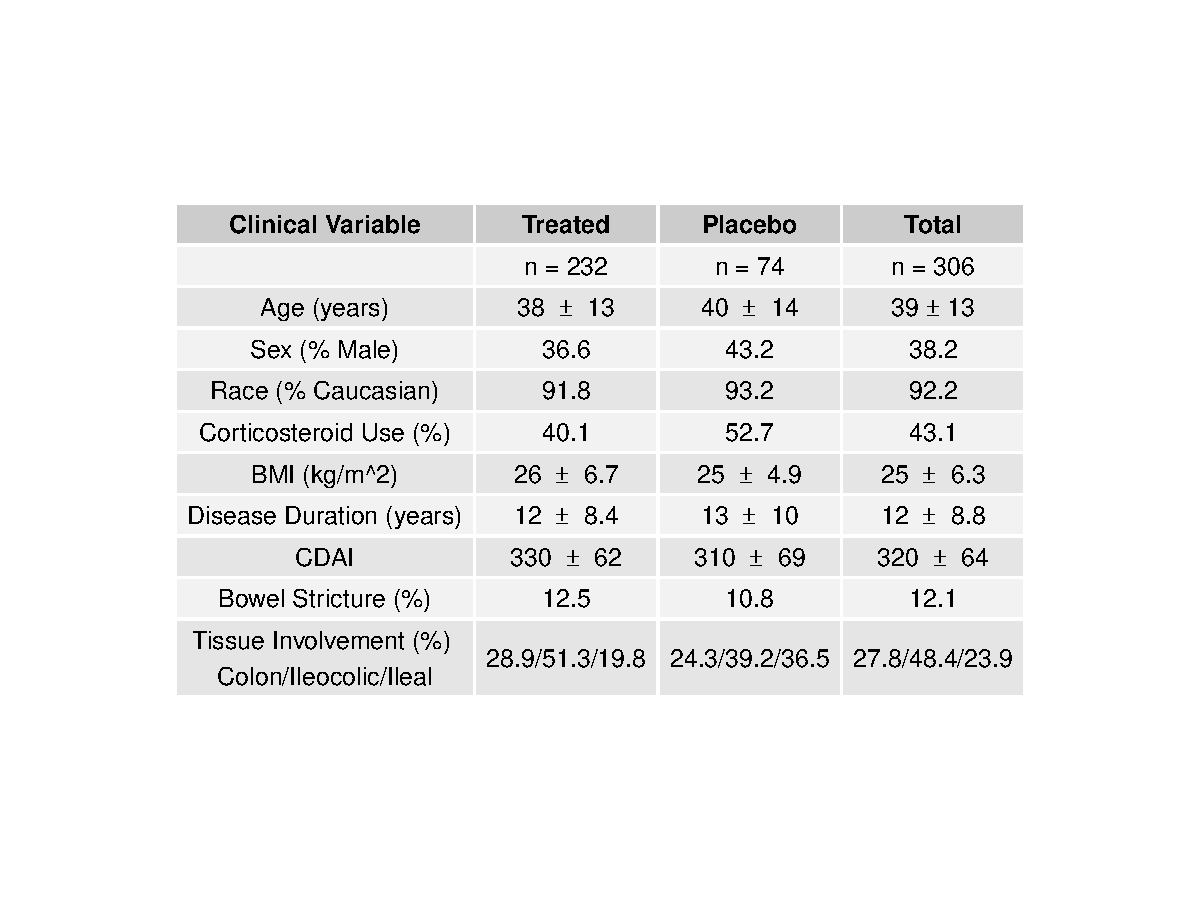
\includegraphics{tables/Table1_baseline_metadata.pdf}

\newpage

\textbf{Supplemental Table 1: Diversity differences based on clinical
metadata of chort at baseline}

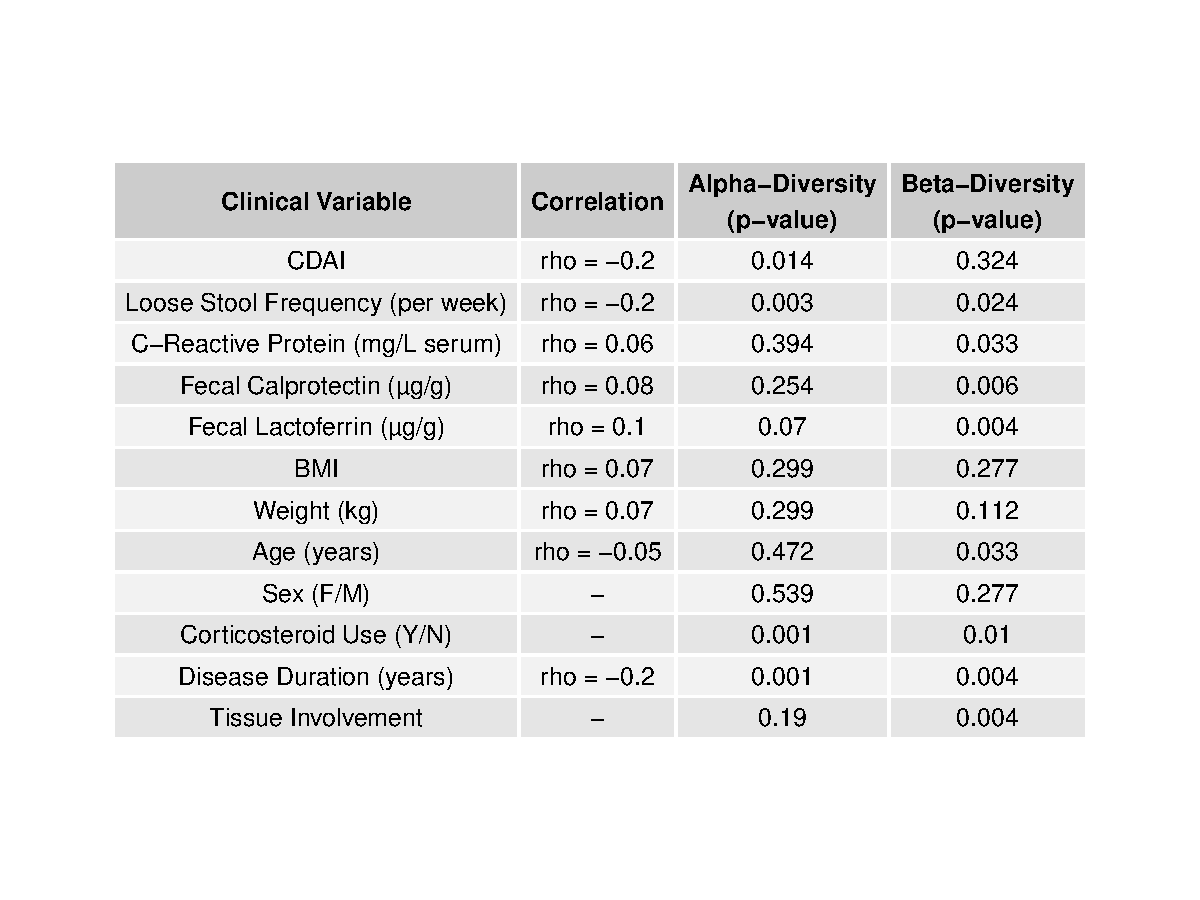
\includegraphics{tables/Supp.table1_cohortdiversity.pdf}

\newpage

\subsection{Figures}\label{figures}

\textbf{Figure 1: Experimental design as adapted from Sanborne et al
2012.} (A) Diagram of experimental design. Participants were divided
into 4 groups of 125 individuals receiving placebo or 1, 3, or 6 mg/kg
doses of UST by IV. At week 8, patients were divided into groups
receiving either subcutaneous injection of UST or placebo at weeks 8 and
16 as maintenance therapy, based on response at week 6. Finally, at 22
weeks patients were scored using CDAI for their response to therapy. (B)
Stool sampling, treatment, and response evalution timeline.

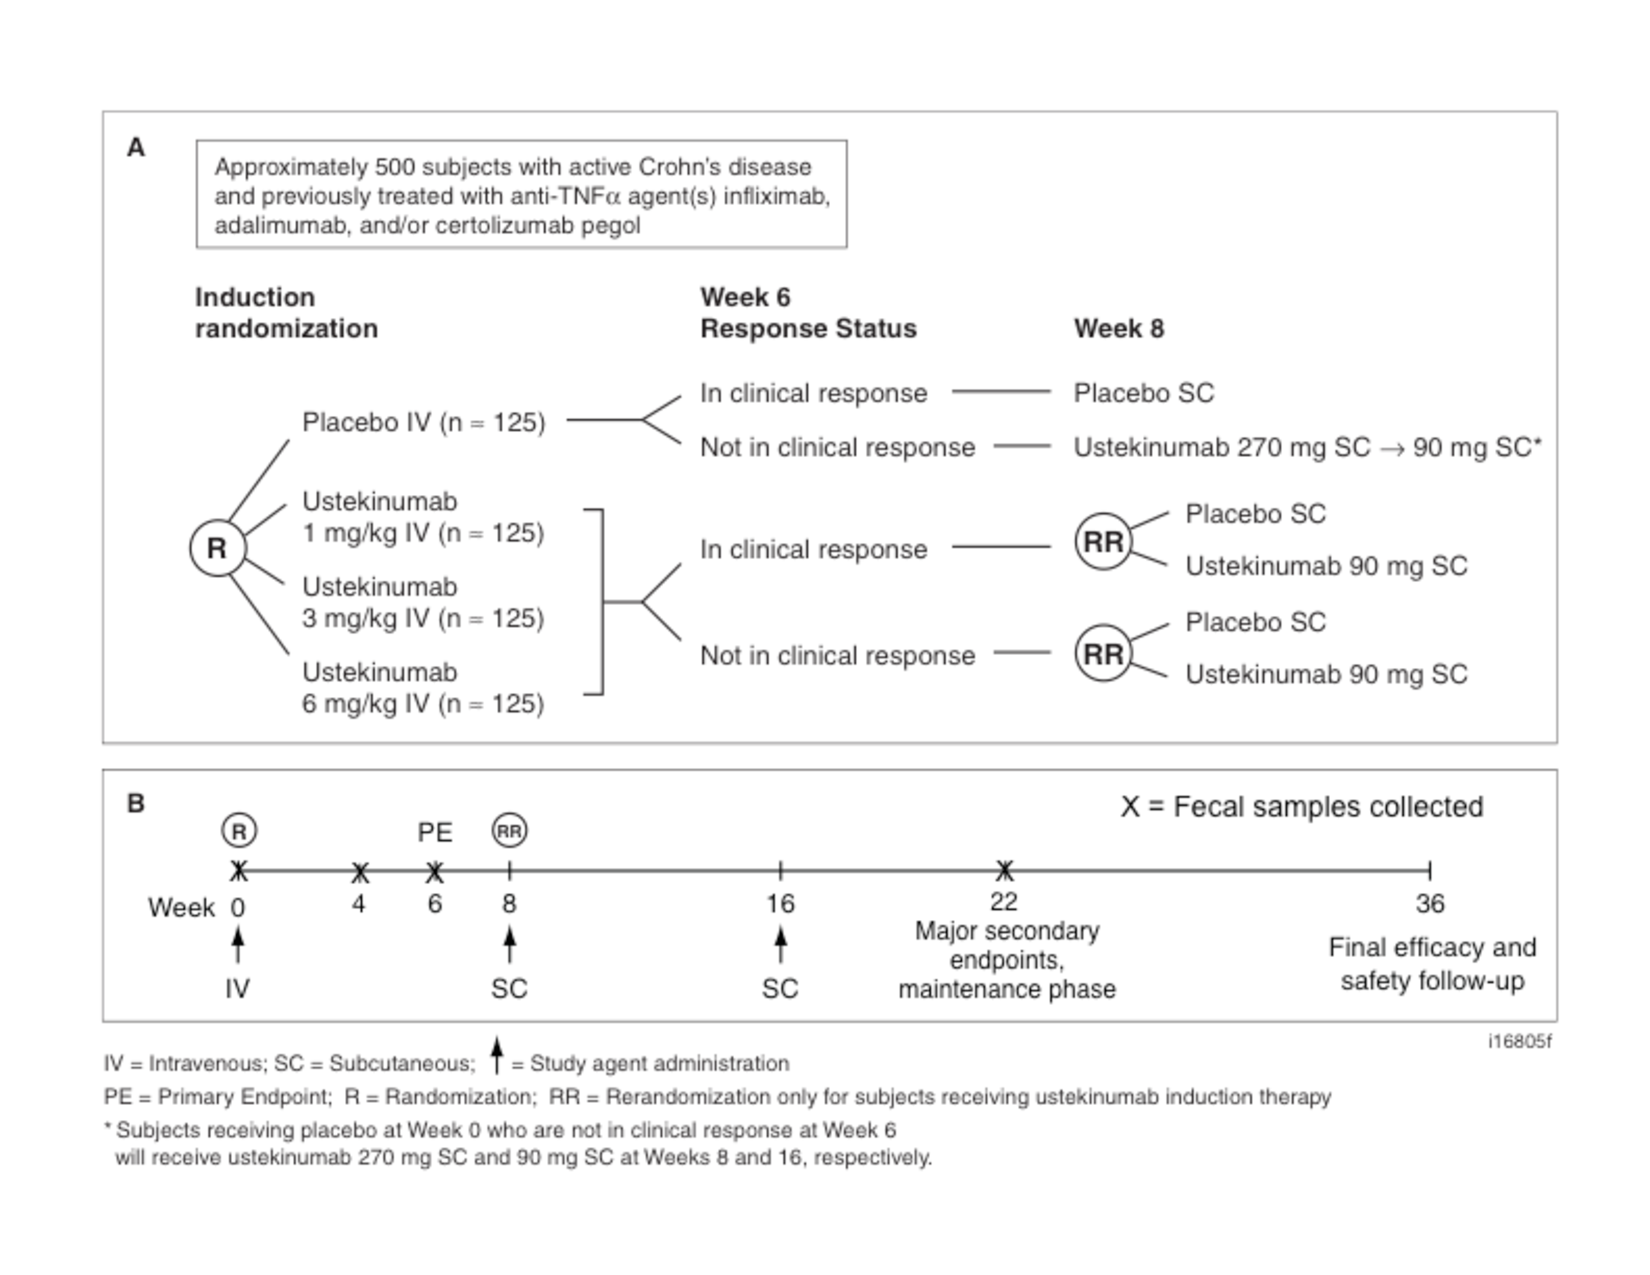
\includegraphics{figures/Figure1_expdesign.pdf}

\newpage

\textbf{Figure 2: Change in alpha diversity over time by induction
treatment and week 22 response status.} The \({\alpha}\)-diversity of 48
subjects induced and maintained with UST and 14 subjects induced and
maintained with placebo was assess at each time point. Friedman test
were perfomed within each teatment and responder group. * indicates week
22 is significantly different from week 0 (p \textless{}0.05).

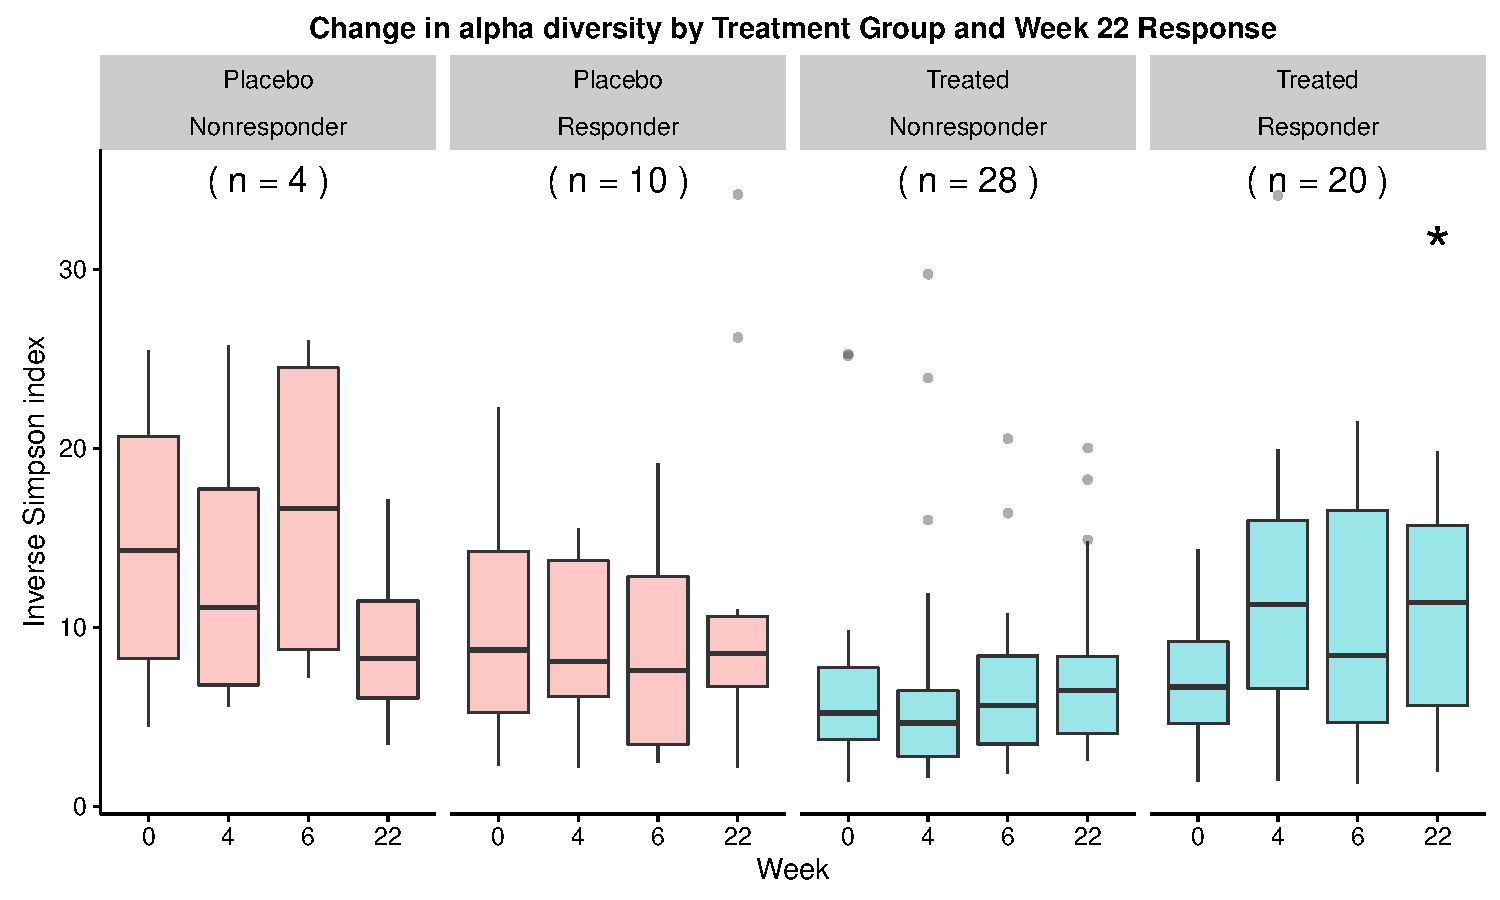
\includegraphics{figures/Figure2_alltp.adivXvisitXindtrtXrelRSPwk22.pdf}

\newpage

\textbf{Figure 3: Classification of week 6 response or remission status
using week 6 stool samples from subjects treated with UST} (A) ROCs for
week 6 outcome based on the week 6 microbiome. (B) Top predictive taxa
from week 6 stool for remission status at week 6, based on MDA.

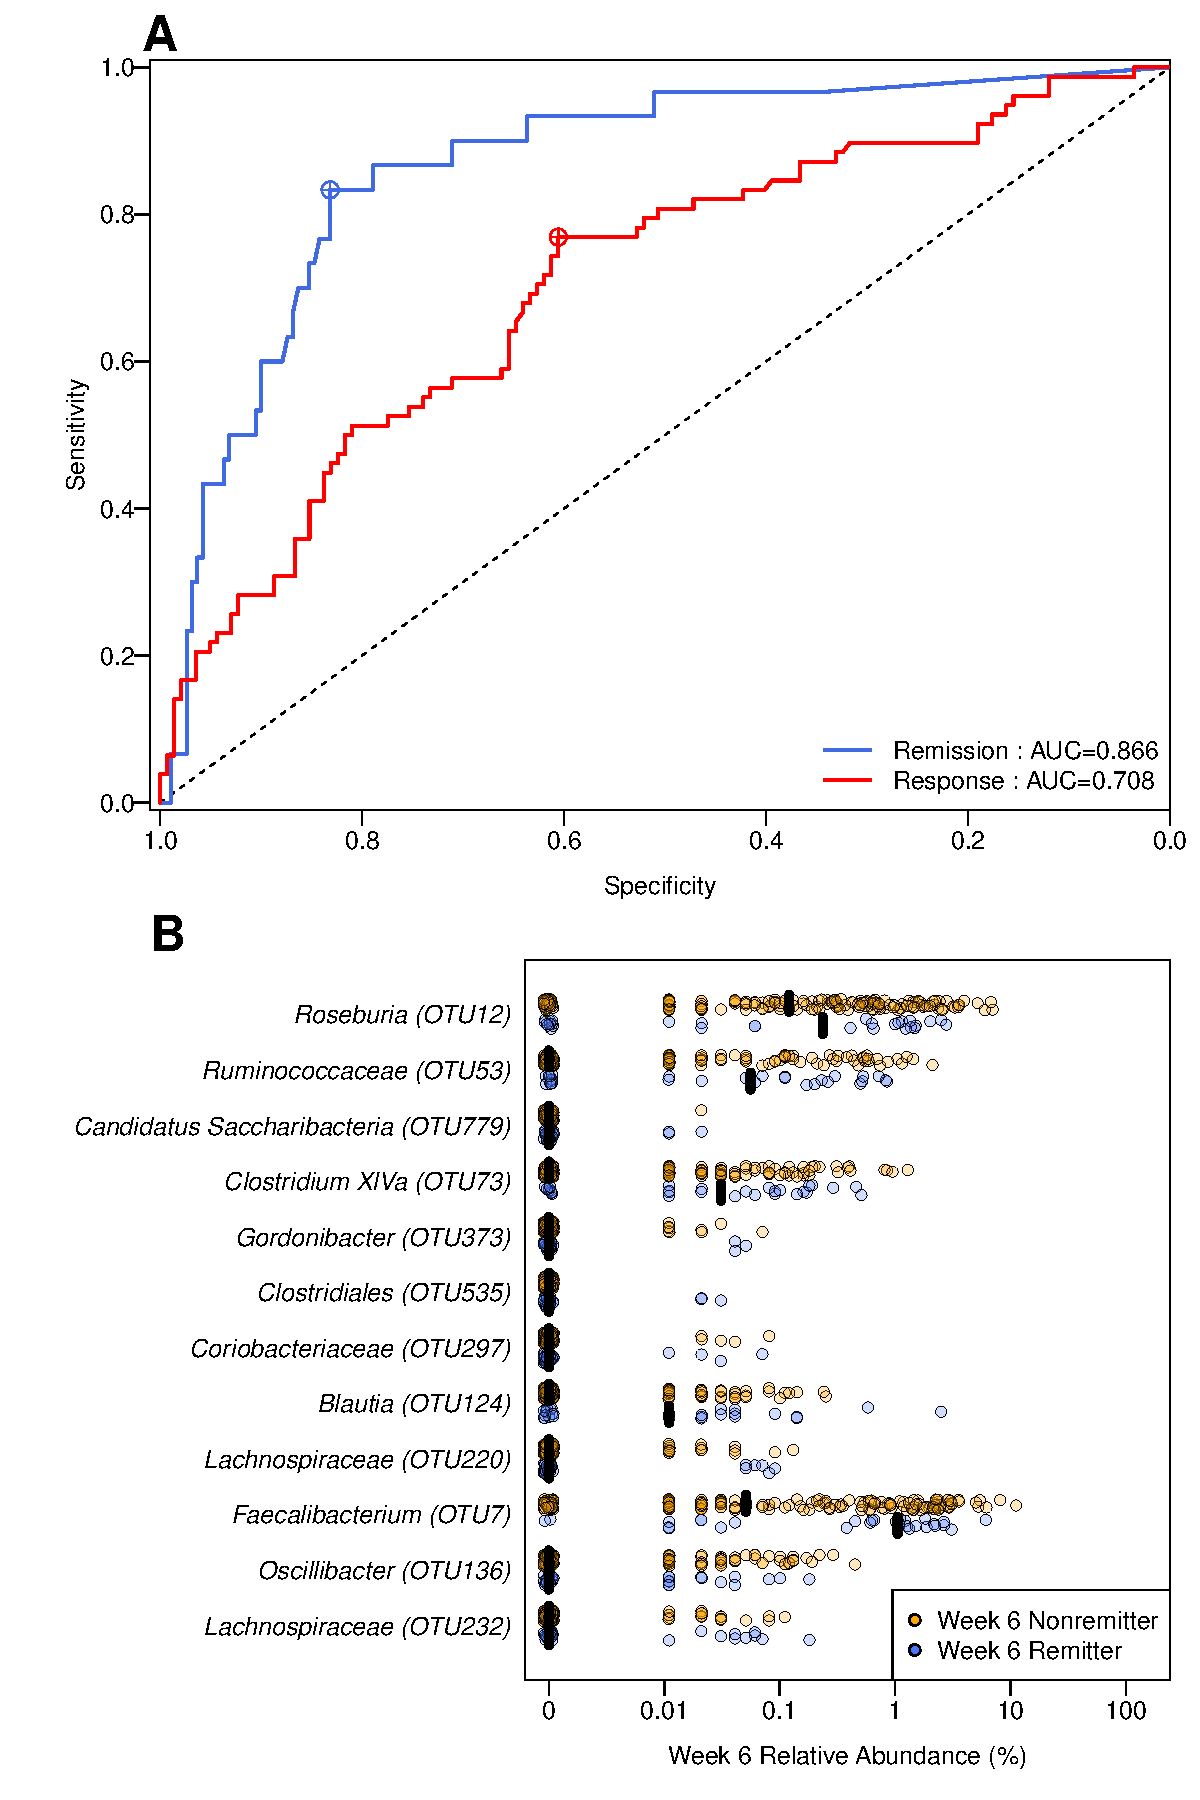
\includegraphics{figures/Figure3_wk6Xwk6.pdf}

\newpage

\textbf{Figure 4: Prediction of week 6 disease status in subjects
treated with UST, using week 0 samples} ROCs for (A) response and (C)
remission using microbiome data, clinical metadata, and a combined
model. Top predictive taxa for the microbiome model based on MDA for (B)
response and (D) remission.

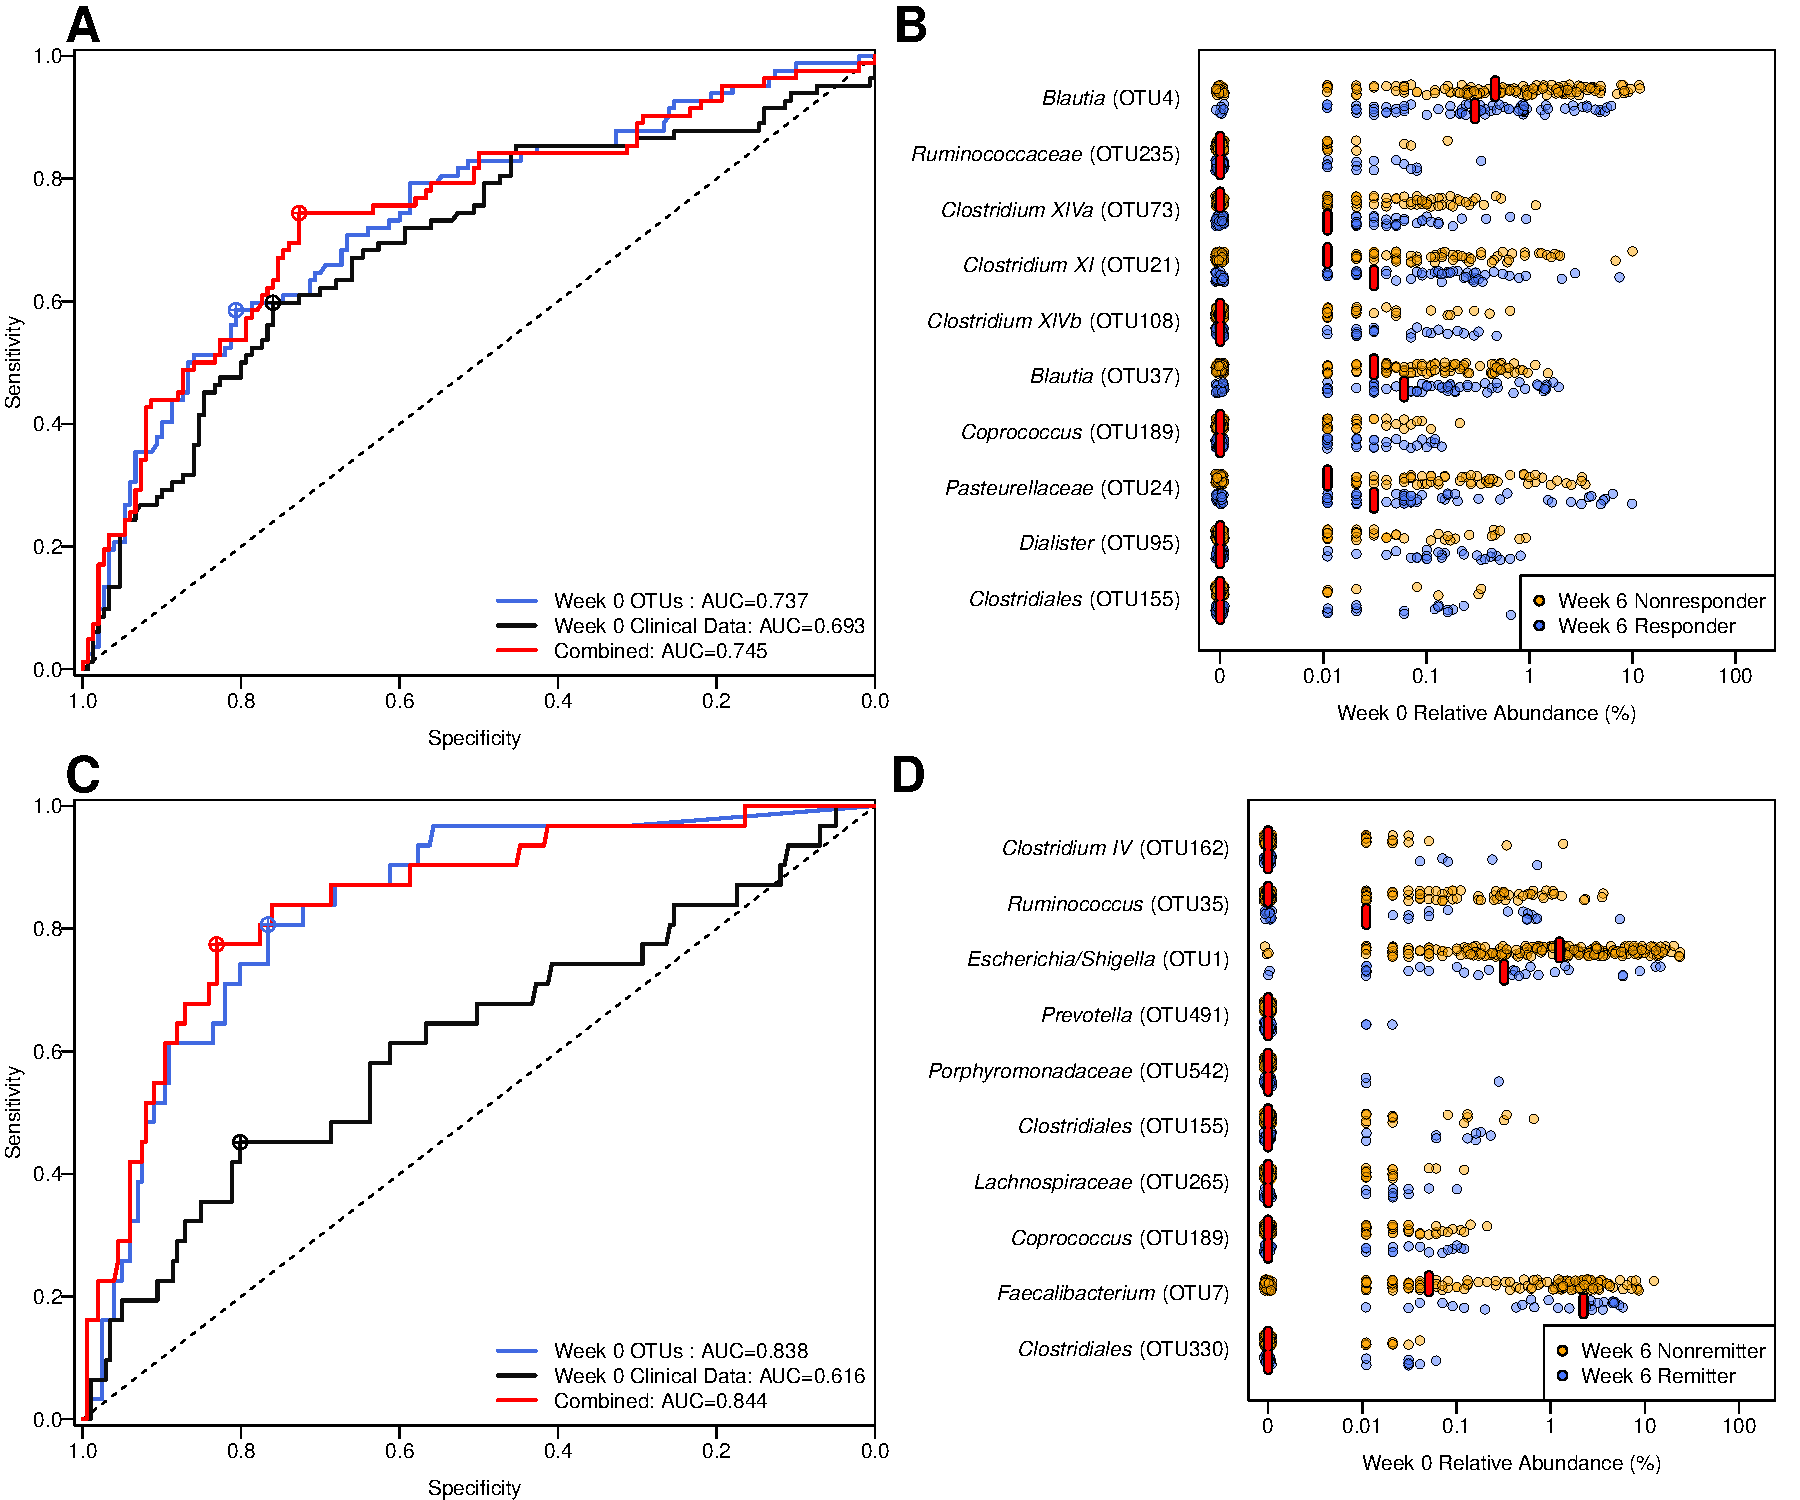
\includegraphics{figures/Figure4_wk0Xwk6pred.pdf}

\newpage

\textbf{Supplemental Figure 1: Phyla from week 0 stool samples in
subjects treated with UST by week 6 outcome} Compared the relative
abundance of each phylum in UST teated subjects based on (A) response
and (B) remission status using a Wilcoxon rank sum test and to identify
phyla where there was a p-value less than 0.05 following a
Benjamini-Hochberg correction for multiple comparisons.

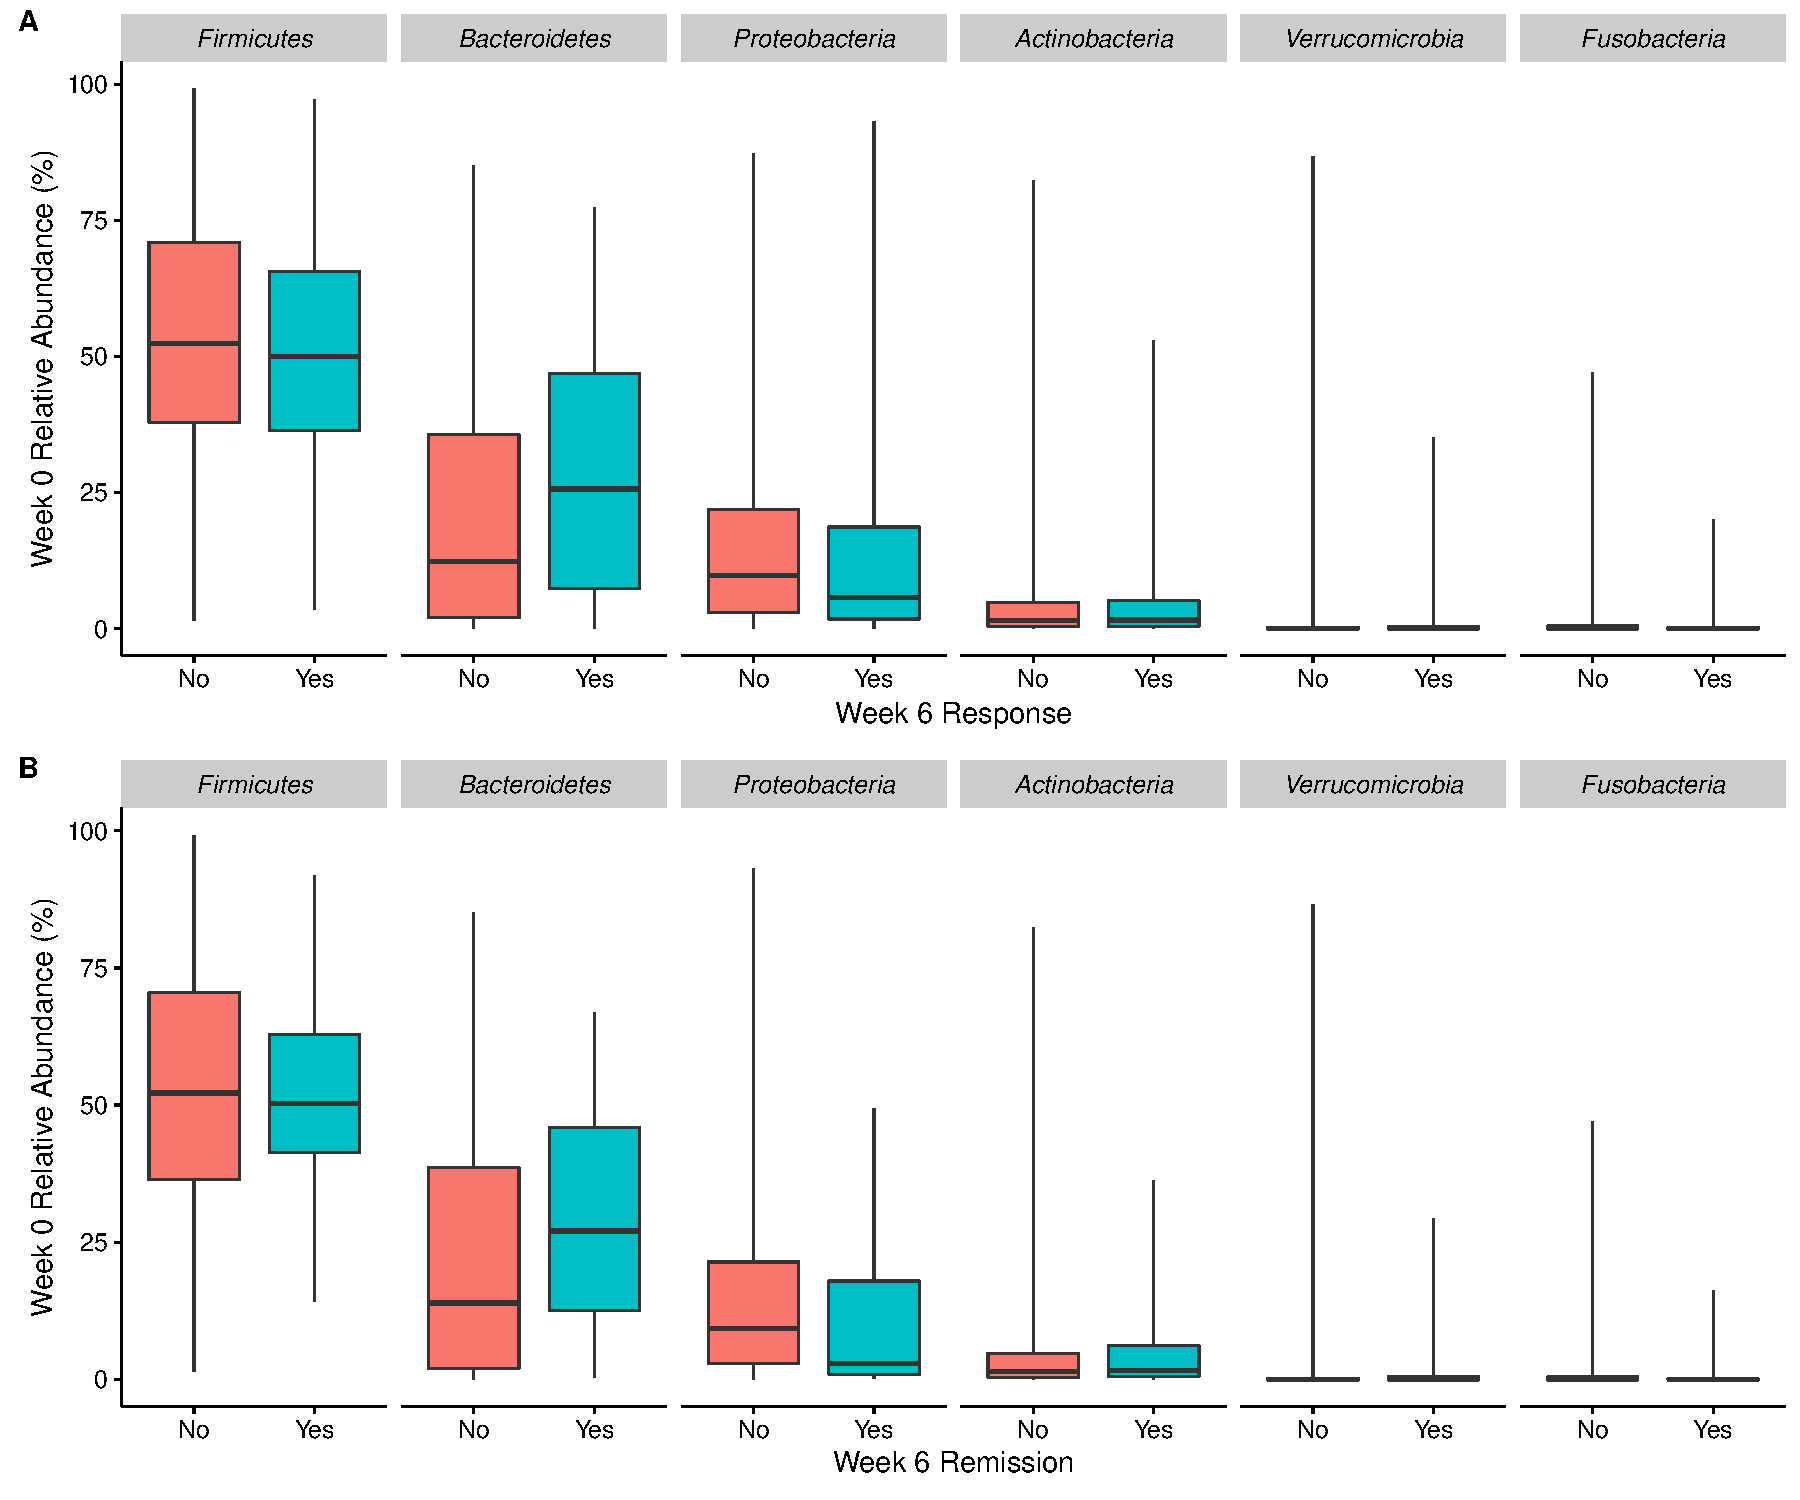
\includegraphics{figures/SF1_wk6phyla.pdf}

\newpage

\textbf{Figure 5: Differential taxa in week 0 stool samples from
subjects treated with UST, based on week 6 remission status} Compared
the relative abundance of each OTU in UST teated subjects based on (A)
response and (B) remission status using a Wilcoxon rank sum test to
identify OTUs where there was a p-value less than 0.05 following a
Benjamini-Hochberg correction for multiple comparisons.

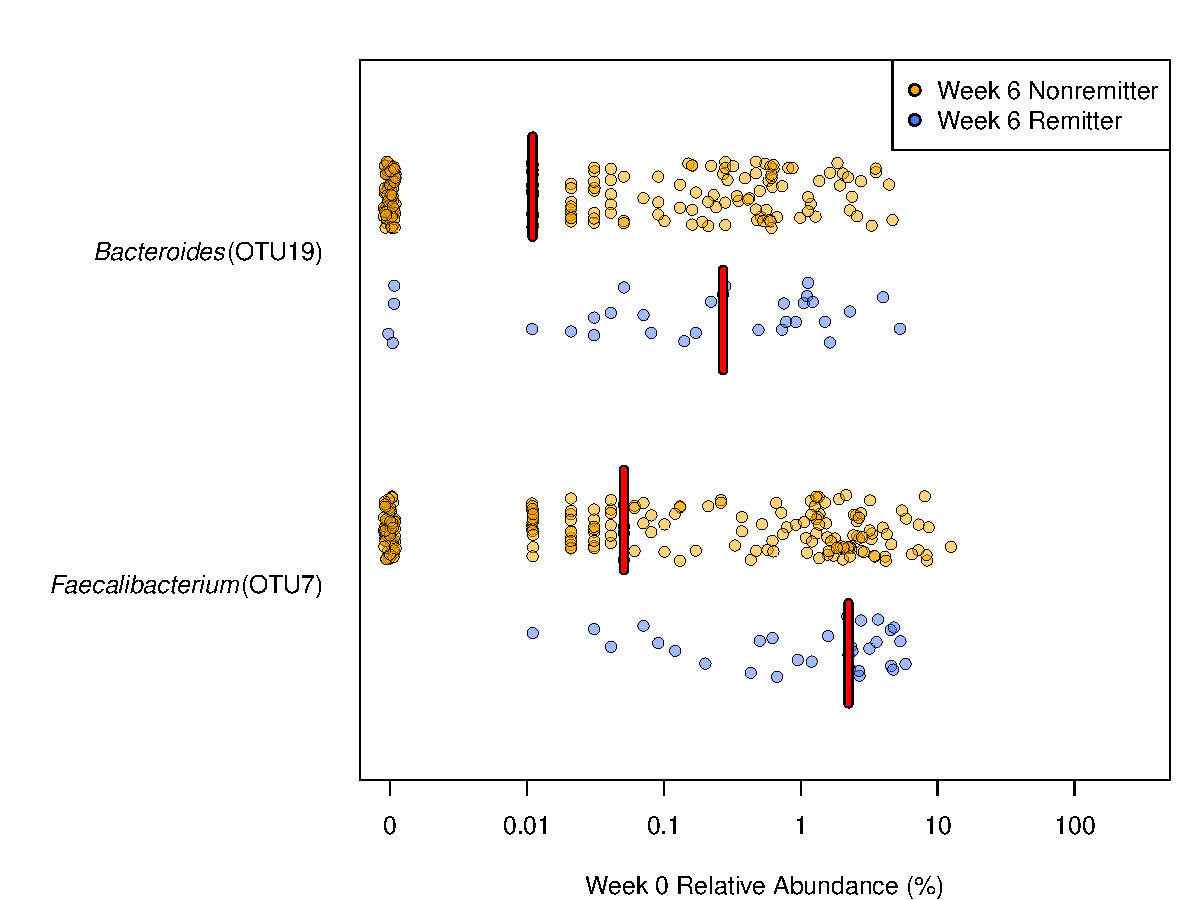
\includegraphics{figures/Figure5_basesigOTUabund.REMISSwk6.pdf}

\newpage

\section*{References}\label{references}
\addcontentsline{toc}{section}{References}

\hypertarget{refs}{}
\hypertarget{ref-ananthakrishnan_epidemiology_2015}{}
1. Ananthakrishnan AN. 2015. Epidemiology and risk factors for IBD. Nat
Rev Gastroenterol Hepatol 12:205--217.

\hypertarget{ref-floyd_economicburden_2015}{}
2. Floyd DN, Langham S, Severac HC, Levesque BG. 2015. The economic and
quality-of-life burden of crohn's disease in europe and the united
states, 2000 to 2013: A systematic review. Dig Dis Sci 60:299--312.

\hypertarget{ref-molodecky_increasingIBD_2012}{}
3. Molodecky NA, Soon IS, Rabi DM, Ghali WA, Ferris M, Chernoff G,
Benchimol EI, Panaccione R, Ghosh S, Barkema HW, Kaplan GG. 2012.
Increasing incidence and prevalence of the inflammatory bowel diseases
with time, based on systematic review. Gastroenterology 142:46--54.e42;
quiz e30.

\hypertarget{ref-randall_CDbiologics_2015}{}
4. Randall CW, Vizuete JA, Martinez N, Alvarez JJ, Garapati KV,
Malakouti M, Taboada CM. 2015. From historical perspectives to modern
therapy: A review of current and future biological treatments for
crohn's disease. Therap Adv Gastroenterol 8:143--59.

\hypertarget{ref-wils_ust_2015}{}
5. Wils P, Bouhnik Y, Michetti P, Flourie B, Brixi H, Bourrier A, Allez
M, Duclos B, Grimaud JC, Buisson A, Amiot A, Fumery M, Roblin X,
Peyrin-Biroulet L, Filippi J, Bouguen G, Abitbol V, Coffin B, Simon M,
Laharie D, Pariente B. 2015. Subcutaneous ustekinumab provides clinical
benefit for two-thirds of patients with crohn's disease refractory to
anti-tumor necrosis factor agents. Clin Gastroenterol Hepatol.

\hypertarget{ref-colombel_deepremission_2015}{}
6. Colombel JF, Reinisch W, Mantzaris GJ, Kornbluth A, Rutgeerts P, Tang
KL, Oortwijn A, Bevelander GS, Cornillie FJ, Sandborn WJ. 2015.
Randomised clinical trial: Deep remission in biologic and
immunomodulator naive patients with crohn's disease - a SONIC post hoc
analysis. Aliment Pharmacol Ther 41:734--46.

\hypertarget{ref-baert_mucosalhealing_2010}{}
7. Baert F, Moortgat L, Van Assche G, Caenepeel P, Vergauwe P, De Vos M,
Stokkers P, Hommes D, Rutgeerts P, Vermeire S, D'Haens G. 2010. Mucosal
healing predicts sustained clinical remission in patients with
early-stage crohn's disease. Gastroenterology 138:463--8; quiz e10--1.

\hypertarget{ref-Lichtenstein_biomarkers_2010}{}
8. Lichtenstein GR. 2010. Emerging prognostic markers to determine
crohn's disease natural history and improve management strategies: A
review of recent literature. Gastroenterol Hepatol (N Y) 6:99--107.

\hypertarget{ref-Chang_biomarkers_2015}{}
9. Chang S, Malter L, Hudesman D. 2015. Disease monitoring in
inflammatory bowel disease. World J Gastroenterol 21:11246--59.

\hypertarget{ref-Boon_biomarkers_2015}{}
10. Boon GJ, Day AS, Mulder CJ, Gearry RB. 2015. Are faecal markers good
indicators of mucosal healing in inflammatory bowel disease? World J
Gastroenterol 21:11469--80.

\hypertarget{ref-Falvey_biomarkers_2015}{}
11. Falvey JD, Hoskin T, Meijer B, Ashcroft A, Walmsley R, Day AS,
Gearry RB. 2015. Disease activity assessment in ibd: Clinical indices
and biomarkers fail to predict endoscopic remission. Inflamm Bowel Dis
21:824--31.

\hypertarget{ref-sartor_IBDpath_2006}{}
12. Sartor RB. 2006. Mechanisms of disease: Pathogenesis of crohn's
disease and ulcerative colitis. Nat Clin Pract Gastroenterol Hepatol
3:390--407.

\hypertarget{ref-wright_CDmicrobiome_2015}{}
13. Wright EK, Kamm MA, Teo SM, Inouye M, Wagner J, Kirkwood CD. 2015.
Recent advances in characterizing the gastrointestinal microbiome in
crohn's disease: A systematic review. Inflamm Bowel Dis 21:1219--28.

\hypertarget{ref-manichanh_diversityCD_2006}{}
14. Manichanh C, Rigottier-Gois L, Bonnaud E, Gloux K, Pelletier E,
Frangeul L, Nalin R, Jarrin C, Chardon P, Marteau P, Roca J, Dore J.
2006. Reduced diversity of faecal microbiota in crohn's disease revealed
by a metagenomic approach. Gut 55:205--11.

\hypertarget{ref-hansen_pedsIBD_2012}{}
15. Hansen R, Russell RK, Reiff C, Louis P, McIntosh F, Berry SH,
Mukhopadhya I, Bisset WM, Barclay AR, Bishop J, Flynn DM, McGrogan P,
Loganathan S, Mahdi G, Flint HJ, El-Omar EM, Hold GL. 2012. Microbiota
of de-novo pediatric IBD: Increased faecalibacterium prausnitzii and
reduced bacterial diversity in crohn's but not in ulcerative colitis. Am
J Gastroenterol 107:1913--22.

\hypertarget{ref-haberman_pedsCD_2014}{}
16. Haberman Y, Tickle TL, Dexheimer PJ, Kim MO, Tang D, Karns R,
Baldassano RN, Noe JD, Rosh J, Markowitz J, Heyman MB, Griffiths AM,
Crandall WV, Mack DR, Baker SS, Huttenhower C, Keljo DJ, Hyams JS,
Kugathasan S, Walters TD, Aronow B, Xavier RJ, Gevers D, Denson LA.
2014. Pediatric crohn disease patients exhibit specific ileal
transcriptome and microbiome signature. J Clin Invest 124:3617--33.

\hypertarget{ref-gevers_pedsCD_2014}{}
17. Gevers D, Kugathasan S, Denson LA, Vazquez-Baeza Y, Van Treuren W,
Ren B, Schwager E, Knights D, Song SJ, Yassour M, Morgan XC, Kostic AD,
Luo C, Gonzalez A, McDonald D, Haberman Y, Walters T, Baker S, Rosh J,
Stephens M, Heyman M, Markowitz J, Baldassano R, Griffiths A, Sylvester
F, Mack D, Kim S, Crandall W, Hyams J, Huttenhower C, Knight R, Xavier
RJ. 2014. The treatment-naive microbiome in new-onset crohn's disease.
Cell Host Microbe 15:382--92.

\hypertarget{ref-Riol-Blanco_IL23microbiome_2010}{}
18. Riol-Blanco L, Lazarevic V, Awasthi A, Mitsdoerffer M, Wilson BS,
Croxford A, Waisman A, Kuchroo VK, Glimcher LH, Oukka M. 2010. IL-23
receptor regulates unconventional il-17-producing t cells that control
infection1. J Immunol 184:1710--20.

\hypertarget{ref-Round_IL23microbiome_2009}{}
19. Round JL, Mazmanian SK. 2009. The gut microbiome shapes intestinal
immune responses during health and disease. Nat Rev Immunol 9:313--23.

\hypertarget{ref-Eken_IL23CD_2014}{}
20. Eken A, Singh AK, Oukka M. 2014. INTERLEUKIN 23 in crohn'S disease.
Inflamm Bowel Dis 20:587--95.

\hypertarget{ref-Shih_IL23Th17_2014}{}
21. Shih VFS, Cox J, Kljavin NM, Dengler HS, Reichelt M, Kumar P,
Rangell L, Kolls JK, Diehl L, Ouyang W, Ghilardi N. 2014. Homeostatic
il-23 receptor signaling limits th17 response through il-22--mediated
containment of commensal microbiota. Proc Natl Acad Sci U S A
111:13942--7.

\hypertarget{ref-Naser_NOD2IL23R_2012}{}
22. Naser SA, Arce M, Khaja A, Fernandez M, Naser N, Elwasila S,
Thanigachalam S. 2012. Role of atg16l, nod2 and il23r in crohn's disease
pathogenesis. World J Gastroenterol 18:412--24.

\hypertarget{ref-Knights_IBDpath_2013}{}
23. Knights D, Lassen KG, Xavier RJ. 2013. Advances in inflammatory
bowel disease pathogenesis: Linking host genetics and the microbiome.
Gut 62:1505--10.

\hypertarget{ref-Huttenhower_IBD_2014}{}
24. Huttenhower C, Kostic AD, Xavier RJ. 2014. Inflammatory bowel
disease as a model for translating the microbiome. Immunity 40:843--54.

\hypertarget{ref-tedjo_CDactivity_2016}{}
25. Tedjo DI, Smolinska A, Savelkoul PH, Masclee AA, Schooten FJ van,
Pierik MJ, Penders J, Jonkers DMAE. 2016. The fecal microbiota as a
biomarker for disease activity in crohn's disease. Scientific Reports,
Published online: 13 October 2016; doi:101038/srep35216.

\hypertarget{ref-Huang_gingivitis_2014}{}
26. Huang S, Li R, Zeng X, He T, Zhao H, Chang A, Bo C, Chen J, Yang F,
Knight R, Liu J, Davis C, Xu J. 2014. Predictive modeling of gingivitis
severity and susceptibility via oral microbiota. ISME J 8:1768--80.

\hypertarget{ref-Wang_cvdrisk_2016}{}
27. Wang Y, Ames NP, Tun HM, Tosh SM, Jones PJ, Khafipour E. 2016. High
molecular weight barley β-glucan alters gut microbiota toward reduced
cardiovascular disease risk. Front Microbiol 7.

\hypertarget{ref-Schubert_cdiff_2016}{}
28. Schubert AM, Sinani H, Schloss PD. 2015. Antibiotic-induced
alterations of the murine gut microbiota and subsequent effects on
colonization resistance against clostridium difficile. MBio 6:e00974.

\hypertarget{ref-Schubert_cdiff_2014}{}
29. Schubert AM, Rogers MAM, Ring C, Mogle J, Petrosino JP, Young VB,
Aronoff DM, Schloss PD. 2014. Microbiome data distinguish patients with
clostridium difficile infection and non-c. difficile-associated diarrhea
from healthy controls. mBio 5.

\hypertarget{ref-Seekatz_cdiff_2016}{}
30. Seekatz AM, Rao K, Santhosh K, Young VB. 2016. Dynamics of the fecal
microbiome in patients with recurrent and nonrecurrent clostridium
difficile infection. Genome Med 8.

\hypertarget{ref-zackular_CRC_2014}{}
31. Zackular JP, Rogers MA, Ruffin MT th, Schloss PD. 2014. The human
gut microbiome as a screening tool for colorectal cancer. Cancer Prev
Res (Phila) 7:1112--21.

\hypertarget{ref-baxter_FIT_2016}{}
32. Baxter NT, Ruffin MT th, Rogers MA, Schloss PD. 2016.
Microbiota-based model improves the sensitivity of fecal immunochemical
test for detecting colonic lesions. Genome Med 8:37.

\hypertarget{ref-wang_pedsCD_2016}{}
33. Wang F, Kaplan JL, Gold BD, Bhasin MK, Ward NL, Kellermayer R,
Kirschner BS, Heyman MB, Dowd SE, Cox SB, Dogan H, Steven B, Ferry GD,
Cohen SA, Baldassano RN, Moran CJ, Garnett EA, Drake L, Otu HH, Mirny
LA, Libermann TA, Winter HS, Korolev KS. 2016. Detecting microbial
dysbiosis associated with pediatric crohn disease despite the high
variability of the gut microbiota. Cell Rep.

\hypertarget{ref-Ananthakrishnan_IBD_2017}{}
34. Ananthakrishnan AN, Luo C, Yajnik V, Khalili H, Garber JJ, Stevens
BW, Cleland T, Xavier RJ. 2017. Gut microbiome function predicts
response to anti-integrin biologic therapy in inflammatory bowel
diseases. Cell Host Microbe 21:603--610.e3.

\hypertarget{ref-Shaw_response_2016}{}
35. Shaw KA, Bertha M, Hofmekler T, Chopra P, Vatanen T, Srivatsa A,
Prince J, Kumar A, Sauer C, Zwick ME, Satten GA, Kostic AD, Mulle JG,
Xavier RJ, Kugathasan S. 2016. Dysbiosis, inflammation, and response to
treatment: A longitudinal study of pediatric subjects with newly
diagnosed inflammatory bowel disease. Genome Med 8:75.

\hypertarget{ref-sandborn_ust_2012}{}
36. Sandborn WJ, Gasink C, Gao LL, Blank MA, Johanns J, Guzzo C, Sands
BE, Hanauer SB, Targan S, Rutgeerts P, Ghosh S, Villiers WJ de,
Panaccione R, Greenberg G, Schreiber S, Lichtiger S, Feagan BG. 2012.
Ustekinumab induction and maintenance therapy in refractory crohn's
disease. N Engl J Med 367:1519--28.

\hypertarget{ref-sandborn_ust_2008}{}
37. Sandborn WJ, Feagan BG, Fedorak RN, Scherl E, Fleisher MR, Katz S,
Johanns J, Blank M, Rutgeerts P. 2008. A randomized trial of
ustekinumab, a human interleukin-12/23 monoclonal antibody, in patients
with moderate-to-severe crohn's disease. Gastroenterology 135:1130--41.

\hypertarget{ref-kopylov_ust_2014}{}
38. Kopylov U, Afif W, Cohen A, Bitton A, Wild G, Bessissow T, Wyse J,
Al-Taweel T, Szilagyi A, Seidman E. 2014. Subcutaneous ustekinumab for
the treatment of anti-TNF resistant crohn's disease--the McGill
experience. J Crohns Colitis 8:1516--22.

\hypertarget{ref-schloss_mothur_2009}{}
39. Schloss PD, Westcott SL, Ryabin T, Hall JR, Hartmann M, Hollister
EB, Lesniewski RA, Oakley BB, Parks DH, Robinson CJ, Sahl JW, Stres B,
Thallinger GG, Van Horn DJ, Weber CF. 2009. Introducing mothur:
Open-source, platform-independent, community-supported software for
describing and comparing microbial communities. Appl Environ Microbiol
75:7537--41.

\hypertarget{ref-calle_aucrf_2011}{}
40. Calle ML, Urrea V, Boulesteix A-L, Malats N. 2011. AUC-RF: A new
strategy for genomic profiling with random forest. Human Heredity
72:121--132.

\hypertarget{ref-naftali_tissinvol_2016}{}
41. Naftali T, Reshef L, Kovacs A, Porat R, Amir I, Konikoff FM, Gophna
U. 2016. Distinct microbiotas are associated with ileum-restricted and
colon-involving crohn's disease. Inflamm Bowel Dis 22:293--302.

\hypertarget{ref-sartor_microbesIBD_2016}{}
42. Sartor RB, Wu GD. 2016. Roles for intestinal bacteria, viruses, and
fungi in pathogenesis of inflammatory bowel diseases and therapeutic
approaches. Gastroenterology.

\hypertarget{ref-boon_fmarkers_2015}{}
43. Boon GJ, Day AS, Mulder CJ, Gearry RB. 2015. Are faecal markers good
indicators of mucosal healing in inflammatory bowel disease? World J
Gastroenterol 21:11469--80.

\hypertarget{ref-chang_monitoring_2015}{}
44. Chang S, Malter L, Hudesman D. 2015. Disease monitoring in
inflammatory bowel disease. World J Gastroenterol 21:11246--59.

\hypertarget{ref-papa_pedsIBD_2012}{}
45. Papa E, Docktor M, Smillie C, Weber S, Preheim SP, Gevers D,
Giannoukos G, Ciulla D, Tabbaa D, Ingram J, Schauer DB, Ward DV,
Korzenik JR, Xavier RJ, Bousvaros A, Alm EJ. 2012. Non-invasive mapping
of the gastrointestinal microbiota identifies children with inflammatory
bowel disease. PLoS One 7:e39242.

\hypertarget{ref-vandeputte_stoolcon_2016}{}
46. Vandeputte D, Falony G, Vieira-Silva S, Tito RY, Joossens M, Raes J.
2016. Original article: Stool consistency is strongly associated with
gut microbiota richness and composition, enterotypes and bacterial
growth rates. Gut 65:57--62.

\hypertarget{ref-huang_cort_2015}{}
47. Huang EY, Inoue T, Leone VA, Dalal S, Touw K, Wang Y, Musch MW,
Theriault B, Higuchi K, Donovan S, Gilbert J, Chang EB. 2015. Using
corticosteroids to reshape the gut microbiome: Implications for
inflammatory bowel diseases. Inflamm Bowel Dis 21:963--72.

\hypertarget{ref-monteleone_mongersen_2015}{}
48. Monteleone G, Neurath MF, Ardizzone S, Di Sabatino A, Fantini MC,
Castiglione F, Scribano ML, Armuzzi A, Caprioli F, Sturniolo GC, Rogai
F, Vecchi M, Atreya R, Bossa F, Onali S, Fichera M, Corazza GR, Biancone
L, Savarino V, Pica R, Orlando A, Pallone F. 2015. Mongersen, an oral
SMAD7 antisense oligonucleotide, and crohn's disease. N Engl J Med
372:1104--13.

\hypertarget{ref-monteleone_mongersen_2016}{}
49. Monteleone G, Di Sabatino A, Ardizzone S, Pallone F, Usiskin K, Zhan
X, Rossiter G, Neurath MF. 2016. Impact of patient characteristics on
the clinical efficacy of mongersen (GED-0301), an oral smad7 antisense
oligonucleotide, in active crohn's disease. Aliment Pharmacol Ther
43:717--24.

\hypertarget{ref-ardizzone_mongersen_2016}{}
50. Ardizzone S, Bevivino G, Monteleone G. 2016. Mongersen, an oral
smad7 antisense oligonucleotide, in patients with active crohn's
disease. Therap Adv Gastroenterol 9:527--32.

\hypertarget{ref-orava_short_2013}{}
51. Orava EW, Jarvik N, Shek YL, Sidhu SS, Gariepy J. 2013. A short DNA
aptamer that recognizes TNFalpha and blocks its activity in vitro. ACS
Chem Biol 8:170--8.

\hypertarget{ref-Kozich_MiSeqSOP_2013}{}
52. Kozich JJ, Westcott SL, Baxter NT, Highlander SK, Schloss PD. 2013.
Development of a dual-index sequencing strategy and curation pipeline
for analyzing amplicon sequence data on the miseq illumina sequencing
platform. Appl Environ Microbiol 79:5112--20.

\hypertarget{ref-schloss_PCRartifacts_2011}{}
53. Schloss PD, Gevers D, Westcott SL. 2011. Reducing the effects of PCR
amplification and sequencing artifacts on 16S rRNA-based studies. PLoS
One 6:e27310.

\hypertarget{ref-Quast_silva_2013}{}
54. Quast C, Pruesse E, Yilmaz P, Gerken J, Schweer T, Yarza P, Peplies
J, Glöckner FO. 2013. The silva ribosomal rna gene database project:
Improved data processing and web-based tools. Nucleic Acids Res
41:D590--6.

\hypertarget{ref-edgar_uchime_2011}{}
55. Edgar RC, Haas BJ, Clemente JC, Quince C, Knight R. 2011. UCHIME
improves sensitivity and speed of chimera detection. Bioinformatics
27:2194--200.

\hypertarget{ref-schloss_OTUanalysis_2011}{}
56. Schloss PD, Westcott SL. 2011. Assessing and improving methods used
in operational taxonomic unit-based approaches for 16S rRNA gene
sequence analysis. Appl Environ Microbiol 77:3219--26.

\hypertarget{ref-wang_taxonomy_2007}{}
57. Wang Q, Garrity GM, Tiedje JM, Cole JR. 2007. Naive bayesian
classifier for rapid assignment of rRNA sequences into the new bacterial
taxonomy. Appl Environ Microbiol 73:5261--7.

\hypertarget{ref-R}{}
58. R Core Team. 2016. R: A language and environment for statistical
computing. R Foundation for Statistical Computing, Vienna, Austria.

\hypertarget{ref-sokal_biometrystats_1995}{}
59. Sokal RR, Rohlf FJ. 1995. Biometry: The principles and practice of
statistics in biological research, 3rd ed. Freeman, New York.

\hypertarget{ref-magurran_measuring_2004}{}
60. Magurran AE. 2004. Measuring biological diversity. Blackwell Pub.,
Malden, Ma.

\hypertarget{ref-yue_thetaYC_2005}{}
61. Yue JC, Clayton MK. 2005. A similarity measure based on species
proportions. Communications in Statistics-Theory and Methods
34:2123--2131.

\hypertarget{ref-schloss_commstruct_2008}{}
62. Schloss PD. 2008. Evaluating different approaches that test whether
microbial communities have the same structure. ISME J 2:265--75.

\hypertarget{ref-oksanen_vegan_2016}{}
63. Oksanen J, Blanchet FG, Friendly M, Kindt R, Legendre P, McGlinn D,
Minchin PR, O'Hara RB, Simpson GL, Solymos P, Stevens MHH, Szoecs E,
Wagner H. 2016. Vegan: Community ecology package. r package version
2.4-1.

\hypertarget{ref-friedman_1937}{}
64. Friedman M. 1937. The use of ranks to avoid the assumption of
normality implicit in the analysis of variance. Journal of the American
Statistical Association 32:675--701.

\hypertarget{ref-pgirmess}{}
65. Giraudoux P. 2016. Pgirmess: Data analysis in ecology.

\hypertarget{ref-AUCRF}{}
66. Urrea V, Calle M. 2012. AUCRF: Variable selection with random forest
and the area under the curve.

\hypertarget{ref-breiman_rf_2001}{}
67. Breiman L. 2001. Random forests. Machine Learning 45:5--32.

\hypertarget{ref-Benjamini_Hochberg_1995}{}
68. Benjamini Y, Hochberg Y. 1995. Controlling the false discovery rate:
A practical and powerful approach to multiple testing. Journal of the
Royal Statistical Society Series B (Methodological) 57:289--300.

\hypertarget{ref-ggplot2}{}
69. Wickham H. 2009. Ggplot2: Elegant graphics for data analysis.
Springer-Verlag New York.

\hypertarget{ref-dplyr}{}
70. Wickham H, Francois R. 2016. Dplyr: A grammar of data manipulation.

\hypertarget{ref-pROC}{}
71. Robin X, Turck N, Hainard A, Tiberti N, Lisacek F, Sanchez J-C,
Müller M. 2011. PROC: An open-source package for r and s+ to analyze and
compare roc curves. BMC Bioinformatics 12:77.

\hypertarget{ref-knitr2014}{}
72. Xie Y. 2014. Knitr: A comprehensive tool for reproducible research
in R. \emph{In} Stodden, V, Leisch, F, Peng, RD (eds.), Implementing
reproducible computational research. Chapman; Hall/CRC.

\hypertarget{ref-knitr2015}{}
73. Xie Y. 2015. Dynamic documents with R and knitr, 2nd ed. Chapman;
Hall/CRC, Boca Raton, Florida.

\hypertarget{ref-knitr2017}{}
74. Xie Y. 2017. Knitr: A general-purpose package for dynamic report
generation in r.

\hypertarget{ref-gridExtra}{}
75. Auguie B. 2016. GridExtra: Miscellaneous functions for ``grid''
graphics.

\hypertarget{ref-devtools}{}
76. Wickham H, Chang W. 2016. Devtools: Tools to make developing r
packages easier.

\hypertarget{ref-knitcitations}{}
77. Boettiger C. 2015. Knitcitations: Citations for 'knitr' markdown
files.

\hypertarget{ref-scales}{}
78. Wickham H. 2016. Scales: Scale functions for visualization.

\hypertarget{ref-tidyr}{}
79. Wickham H. 2017. Tidyr: Easily tidy data with 'spread()' and
'gather()' functions.

\hypertarget{ref-Hmisc}{}
80. Harrell Jr FE, Charles Dupont, others. 2016. Hmisc: Harrell
miscellaneous.

\hypertarget{ref-cowplot}{}
81. Wilke CO. 2016. Cowplot: Streamlined plot theme and plot annotations
for 'ggplot2'.


\end{document}
